\documentclass[12pt]{article}%
%Options -- Point size:  10pt (default), 11pt, 12pt
%        -- Paper size:  letterpaper (default), a4paper, a5paper, b5paper
%                        legalpaper, executivepaper
%        -- Orientation  (portrait is the default)
%                        landscape
%        -- Print size:  oneside (default), twoside
%        -- Quality      final(default), draft
%        -- Title page   notitlepage, titlepage(default)
%        -- Columns      onecolumn(default), twocolumn
%        -- Equation numbering (equation numbers on the right is the default)
%                        leqno
%        -- Displayed equations (centered is the default)
%                        fleqn (equations start at the same distance from the right side)
%        -- Open bibliography style (closed is the default)
%                        openbib

% general layout
\usepackage[dvips,letterpaper,margin=0.75in,bottom=0.75in]{geometry}
\usepackage{rotating}
%\usepackage{multicol}
\setlength{\parindent}{0pt}
\usepackage{setspace} % line spacing
\usepackage{changepage}

%\pagestyle{empty} % Removes page numbers
%\pagestyle{plain} 
\usepackage{fancyhdr}
\usepackage{lastpage}
\usepackage{extramarks}

% Setup the header and footer
\fancyhf{}
\pagestyle{fancy}                                                       %
\rhead{Page\ \thepage\ of\ \pageref{LastPage}}                          %
\renewcommand\headrulewidth{0.4pt}                                      %
\renewcommand\footrulewidth{0pt}                                      %

% Make title
\title{\vspace{-1cm}\textmd{\textbf{\hmwkClass:\ \hmwkTitle}}\\\normalsize\vspace{0.1in}\small{Due\ on\ \hmwkDueDate}\\\vspace{0.1in}}
\date{}
\author{\textbf{\hmwkAuthorName}}\vspace{-0.2in}

% base encodings
\usepackage[utf8]{inputenc}
\usepackage[T1]{fontenc}

% math support packages
\usepackage{amsmath}
\usepackage{amsfonts}
\usepackage{amssymb}
\usepackage{mathabx}
%\usepackage[retainorgcmds]{IEEEtran} % problems installing with MikTeX
\DeclareMathOperator{\tr}{tr} % trace of a matrix
\usepackage{mathptmx}
%\usepackage{newtxmath}
\usepackage{bm} % bold math
%\usepackage{commath}
\usepackage{mathtools}
\usepackage{upgreek}
\DeclareMathAlphabet{\mathcal}{OMS}{cmsy}{m}{n}


% graphics-related packages and settings
\usepackage{graphicx}
\graphicspath{ {images/} }
\usepackage{wrapfig} % allow text to wrap around (narrow) figures
%\usepackage{float} % do not use with floatrow
\usepackage{floatrow} % allow floats and captions side by side
\usepackage[font=small,labelfont=bf,labelsep=space,justification=raggedright]{caption}
\usepackage{chngcntr} % defines \counterwithin and \counterwithout
\counterwithin{figure}{section}

% table formatting
\usepackage{makecell}
\usepackage[table]{xcolor}
\usepackage{array} % wrap within tables
\newcolumntype{L}{>{\centering\arraybackslash}m{12cm}}

% miscellaneous
\usepackage{subfiles} % include source from separate files
\usepackage{hyperref} % hypertext support
\usepackage{color}
\usepackage[bottom]{footmisc}
\newcommand{\tsub}[1]{\textsubscript{#1}}
\newcommand{\tsup}[1]{\textsuperscript{#1}}
\newcommand{\so}{\qquad \implies \qquad}
\newcommand{\todo}{\color{red}{TODO}\color{black}\hspace{2mm}}

% for software source code
% Python, Matlab, etc are built in as atandard but Julia needs to be added here
\usepackage{listings}
%%
%% Julia definition (c) 2014 Jubobs
%%
\lstdefinelanguage{Julia} 
{morekeywords={abstract,break,case,catch,const,continue,do,else,elseif,%
		end,export,false,for,function,immutable,import,importall,if,in,%
		macro,module,otherwise,quote,return,switch,true,try,type,typealias,%
		using,while},%
	sensitive=true,%
	alsoother={$},%
	morecomment=[l]\#,%
	morecomment=[n]{\#=}{=\#},%
	morestring=[s]{"}{"},%
	morestring=[m]{'}{'},%
}[keywords,comments,strings]%






%\setlength{\headsep}{-10pt}
\setlength{\parskip}{0.2em}
%\setlength{\textheight}{11 in}
\setlength{\skip\footins}{20pt}

% opening
\title{Plotting large datasets}
\author{Colin Leach, March 2020}
\date{\vspace{-3ex}}

\hyphenpenalty=1000

\begin{document}
	
\maketitle

Galaxy simulations, even undergraduate projects, can involve upwards of $10^7$ particles. Tough to plot, so what are some options?

I made these notes for my own use but there may (?) be other students who are interested.

The dataset used is an array with shape (3, 975000), so 975,000 sets of $(x,y,z)$ coordinates, at a time when two galaxies are tidally disrupting one another.

\section{Static plots}

\subsection{Matplotlib hist2d}

Covered in Lab 7 of ASTR400B, which also adds density contours. That only dealt with single disks but extending it to collisions is relatively simple. Think centering, orientation and (perhaps hardest!) what $x$ and $y$ limits to set.

The result may look something like this:

{\centering 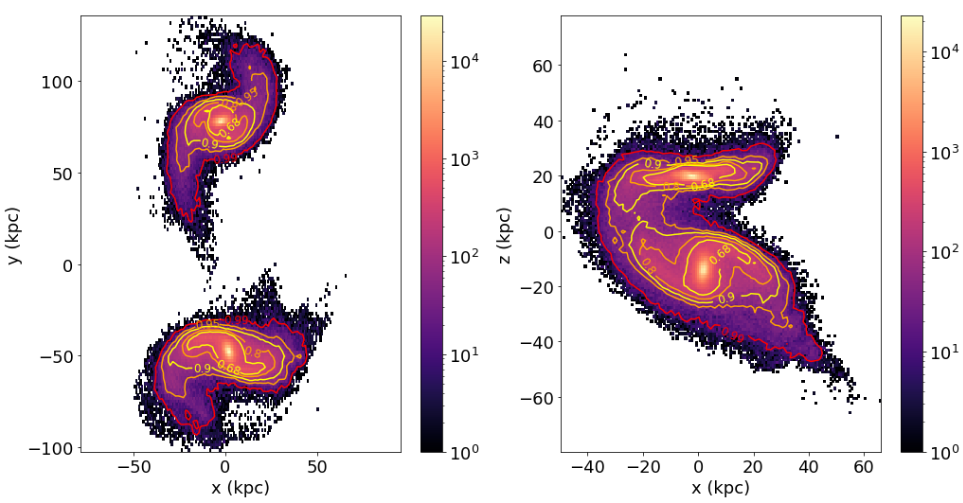
\includegraphics[scale=0.5]{mpl contours, 400b code} \par}

\subsection{Matplotlib plus mpl\_scatter\_density}

This isn't a new problem, so someone wrote an extension to matplotlib to make density plots easier.

Website: \url{https://github.com/astrofrog/mpl-scatter-density}

Borrowing heavily from their examples, this is a first attempt:

\lstdefinestyle{py}{
	belowcaptionskip=1\baselineskip,
	breaklines=true,
	frame=L,
	xleftmargin=\parindent,
	language=Python,
	showstringspaces=false,
	basicstyle=\footnotesize\ttfamily,
	keywordstyle=\bfseries\color{green!40!black},
	commentstyle=\itshape\color{purple!40!black},
	identifierstyle=\color{blue},
	stringstyle=\color{orange},
}

\lstset{style=py} 
\begin{lstlisting}
# install with `conda install mpl-scatter-density`
import mpl_scatter_density

# Make the norm object to define the image stretch
from astropy.visualization import LogStretch
from astropy.visualization.mpl_normalize import ImageNormalize
norm = ImageNormalize(vmin=0., vmax=1000, stretch=LogStretch())

# Make the plot in the (almost) usual pyplot way
# Note the projection to invoke mpl_scatter_density
#  and the norm to use LogStretch

fig = plt.figure(figsize=(12,10))
ax = fig.add_subplot(1, 1, 1, projection='scatter_density')
density = ax.scatter_density(disks[0], disks[1], norm=norm)
plt.xlim(-120, 120)
plt.ylim(-120, 120)

# Add axis labels (standard pyplot)
fontsize = 18
plt.xlabel('x (kpc)', fontsize=fontsize)
plt.ylabel('y (kpc)', fontsize=fontsize)
fig.colorbar(density, label='Number of stars per pixel')
\end{lstlisting}

{\centering 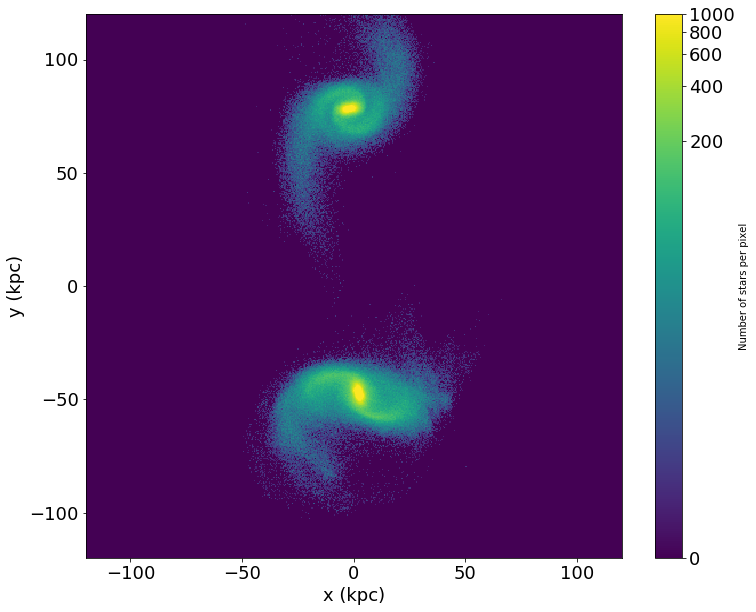
\includegraphics[scale=0.55]{msg} \par}

The colorbar needs some work, but we now get pixel-level resolution. It's a bit easier to see the tidal tails, at least on screen (printouts can be disappointing).

First impressions: a nice addition to matplotlib, quick and easy to set up and use.

\section{Interactive plots}

Getting away from matplotlib, there are some newer\footnote{In other words, typically less finished and poorly documented} options which use the power of modern graphics cards to handle large numbers of points. More powerful, steeper learning curve.

\subsection{datashader}

Websites: \url{https://github.com/holoviz/datashader} and \url{https://datashader.org}

This needs the data to be arranged columnwise in a (single) pandas dataframe; fairly typical for modern plotting packages. Used in isolation, datashader will make a 2D image. To add axes, labels, etc, it needs to be hooked into a suitable browser-based package such as Bokeh (usually) or Plotly (under development). This can mean a LOT of extra packages to install from conda or pip and lots of potential conflicts\footnote{The release of Bokeh 2.0 broke datashader 0.10.0. For now, use Bokeh 1.4.0 and hope datashader 0.13 is released soon. The developer says he's working on it while in self-isolation after flying home from Covid-hit Spain.}

It was a fight for me to get something working. Documentation is extensive, but sometimes out of date and actively misleading (it took over an hour to change the colormap at about the 20th attempt).
The best result so far starts with a bunch of imports:

\begin{lstlisting}
import pandas as pd
import numpy as np
from matplotlib import cm # use the same colormap as other examples

import holoviews as hv
import holoviews.operation.datashader as hd
hv.extension("bokeh") 
hv.output(backend="bokeh")

import datashader as ds
\end{lstlisting}

Then massage the data into the right format and plot it:

\begin{lstlisting}
# convert np.array to pandas dataframe
points_df = pd.DataFrame(disks.T, columns=('x (kpc)','y (kpc)','z (kpc)'))

# convert df to Holoviews points
points = hv.Points(points_df)

# plot in Bokeh
hd.datashade(points, cmap=cm.magma).opts(height=600, width=600)
\end{lstlisting}

The results aren't terrible (see below), but we've still to make the cmap logarithmic, fix the font sizes and add a title. Perhaps another day...

Meanwhile, the best feature is it lets you (in Jupyter) pan with mouse drags and zoom with the mouse wheel or box selection. Matplotlib can't do that so easily (though the ``\%matplotlib notebook'' magic is an option worth knowing about).

{\centering 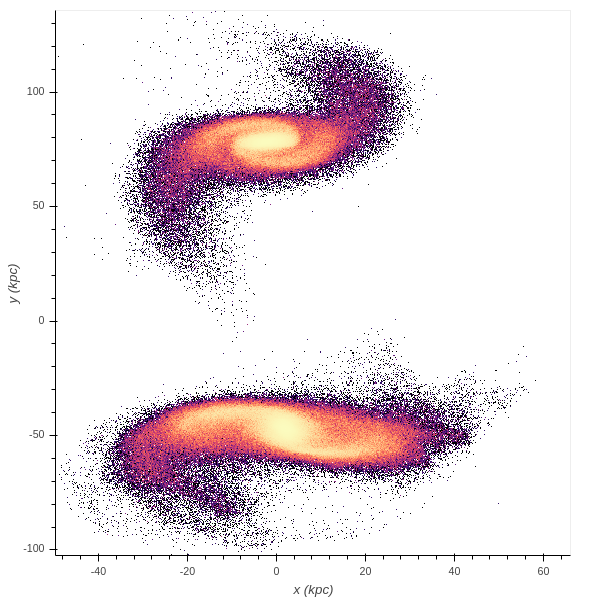
\includegraphics[scale=0.55]{bokeh_datashade} \par}


\subsection{ipyvolume}

Works natively with 3D data. Only in the browser as it relies on WebGL rendering.

Websites: \url{https://github.com/maartenbreddels/ipyvolume} and  \url{https://ipyvolume.readthedocs.io/en/latest/}

Spectacular when the developer (Maarten Breddels, a Dutch astronomer) demonstrates it at conferences, not so easy for the rest of us. I totally failed with this about a year ago, still psyching myself up for another attempt. Anyone else tried it?

\subsection{All things OpenGL}

Now we're at the heavy end of the options. With pyqt5 + (pyopengl or vispy), an experienced graphics programmer with unlimited time can do virtually anything. Though the same person would probably ignore Python and use C++ with GLSL; probably wise, because the C++ libraries at least have good documentation.

I played with this a bit over spring break. At the current rate of progress, I may have a crude prototype working by the end of the Spring 2021 semester (but no promises).

\section{Making movies}

The simplest approach is to make a series of 2D plots then link them in an mp4 file. The NASA movies are clearly much more sophisticated but we don't know how they were made.

\subsection{Within matplotlib}

There are various Animation classes in Matplotlib that can do this: 
\url{https://matplotlib.org/api/animation_api.html}

It's a while since I did this so I don't have a simple working example. Google ``matplotlib animation'' and it will find many blog posts that may be useful.

A personal opinion: this is great for generating simple movies on the fly within Jupyter, for immediate display in the browser. For more serious work I prefer the ffmpeg approach in the next section. You may very well disagree, which is fine.

\subsection{Using ffmpeg}

Matplotlib can export the plot to a PNG or JPEG file and it's easy to write a python loop to produce a bunch of these with names like plot\_000.png, plot\_001.png, etc for the various snaps.

The (HUGE) graphics package ffmpeg can stitch these together into an mp4 movie file. The syntax is something like this (pretty short by ffmpeg standards):

\begin{lstlisting}
ffmpeg -r 10 -start_number 0 -s 1920x1080 -i plot_%03d.png -vcodec libx264 \
  -vf fps=25 -crf 25 -pix_fmt yuv420p my_movie.mp4
\end{lstlisting}

Steps:

\begin{itemize}
	\item Install ffmpeg if it's not already on your system. Linux/Mac users can probably get it from a repository, Windows users (or anyone) can get it from \url{https://ffmpeg.org/download.html}. It works well on Windows.
	\item Make the plot files with names having \textbf{consecutive numbering} and and \textbf{zero-padded to a constant length}. So using a list like 000, 001, 002... is fine, 000, 005, 010... will fail (not consecutive) and 8, 9, 10... will fail (not same length). Can you guess I learned that the hard way? 
	\item In Python, the file names are easy to generate with f-strings:
	\begin{lstlisting}
	 fname = f'plot_{snap:03}.png'
	\end{lstlisting}
	The snap then is padded to 3 digits with leading zeros, and this matches the `\%03d' in the ffmepg command (after the -i switch, for input). To use non-consecutive snaps, keep a separate counter variable:
	\begin{lstlisting}
	for i, snap in enumerate(np.arange(0, 20, 5)):
		# get data for snap, then...
		fname = f'plot_{i:03}.png'	
	\end{lstlisting}
	
	\item The command may take a few attempts to get right. Maybe best assembled in a text editor rather than directly in the command shell. It's really all one line, but line continuation characters are your friend: backslash \textbackslash\ for Linux (and Mac?), carat \^\ for Windows.
	\item Set start\_number for your first file. You can't specify last\_number or step\_by. It stops automatically when it fails to find the next highest number.
	\item Other options (-r, -vf, -crf) are in the ffmeg documentation (good luck!) and many StackExchange posts. I resorted to trial and error.
\end{itemize}

There are other gotchas to fall into. Obviously the $x$ and $y$ limits need to be hard-coded in matplotlib, otherwise the frames will jump about and make you cross-eyed. 

Less obviously, the pixel height of every image must be an even number. Matplotlib doesn't think about that but I found a hack online which seems to work.

\begin{lstlisting}
# The simple figsize format is OK for static images:
# fig = plt.figure(figsize=(20,9))

# If saved files are to be used for animations with ffmpeg, row
# count must be an even number. This hack ensures that.
fig = plt.figure()
DPI = fig.get_dpi() # dots per inch of your display
fig.set_size_inches(1200.0/float(DPI),610.0/float(DPI))
\end{lstlisting}

DPI is 72 on my machine (your result may be different). Make sure your pixel count (1200, 610 in this case) uses even numbers and hope for the best.


\end{document}
